\newpage

\section{Generative and Autoregressive Models}
\subsection{Generative Models}
\subsubsection{Discriminative vs Generative models}
A \emph{discriminative model} is the most common type of supervised learning model: for any input $x$, it predicts its label $y$. Probabilistically speaking, a dscriminative model learns the conditional probability distribution $\P(y|x)$, that is the probability for each label to correspond to the input.

A \emph{generative model} learns the probability distribution $\P(x)$, or in the case of a \emph{conditional generative model}, the conditional distribution $\P(x|y)$, which present a huge mathematical and practical distinction with discriminative models.

Note that a discriminative model has no way to handle \say{unreasonable inputs}: if an input does not fit the training distribution, the model still needs to output a probability distribution over the outputs set. Nevertheless, generative models can predict the likeliness of an input to belong to the input distribution: it can \say{reject} unreasonable inputs by assigning small probabilities to them.

According to Bayes' rule, it is possible to build a conditional generative model from other components:
\begin{equation*}
    \underbrace{\P(x|y)}_{\substack{\text{Conditional}\\ \text{Generative Model}}} = \frac{\overbrace{\P(y|x)}^{\text{Discriminative Model}}}{\underbrace{\P(y)}_{\text{Prior over labels}}}\cdot\underbrace{\P(x)}_{\substack{\text{Unconditional}\\ \text{Generative Model}}}
\end{equation*}
This shows that building an unconditional generative model provides a conditional one without additional complexity.

Generative models can be used for a variety of tasks, including the detection of unlikely inputs, features learning and the generation of new input data by sampling from the learned distribution.

\subsubsection{Taxonomy of generative models}
Various types of generative models have emerged. The main distinctions can be made between models that can compute $\P(x)$ (explicit density models) and models that can only sample from it (implicit density models).
\begin{figure}[H]
    \centering
    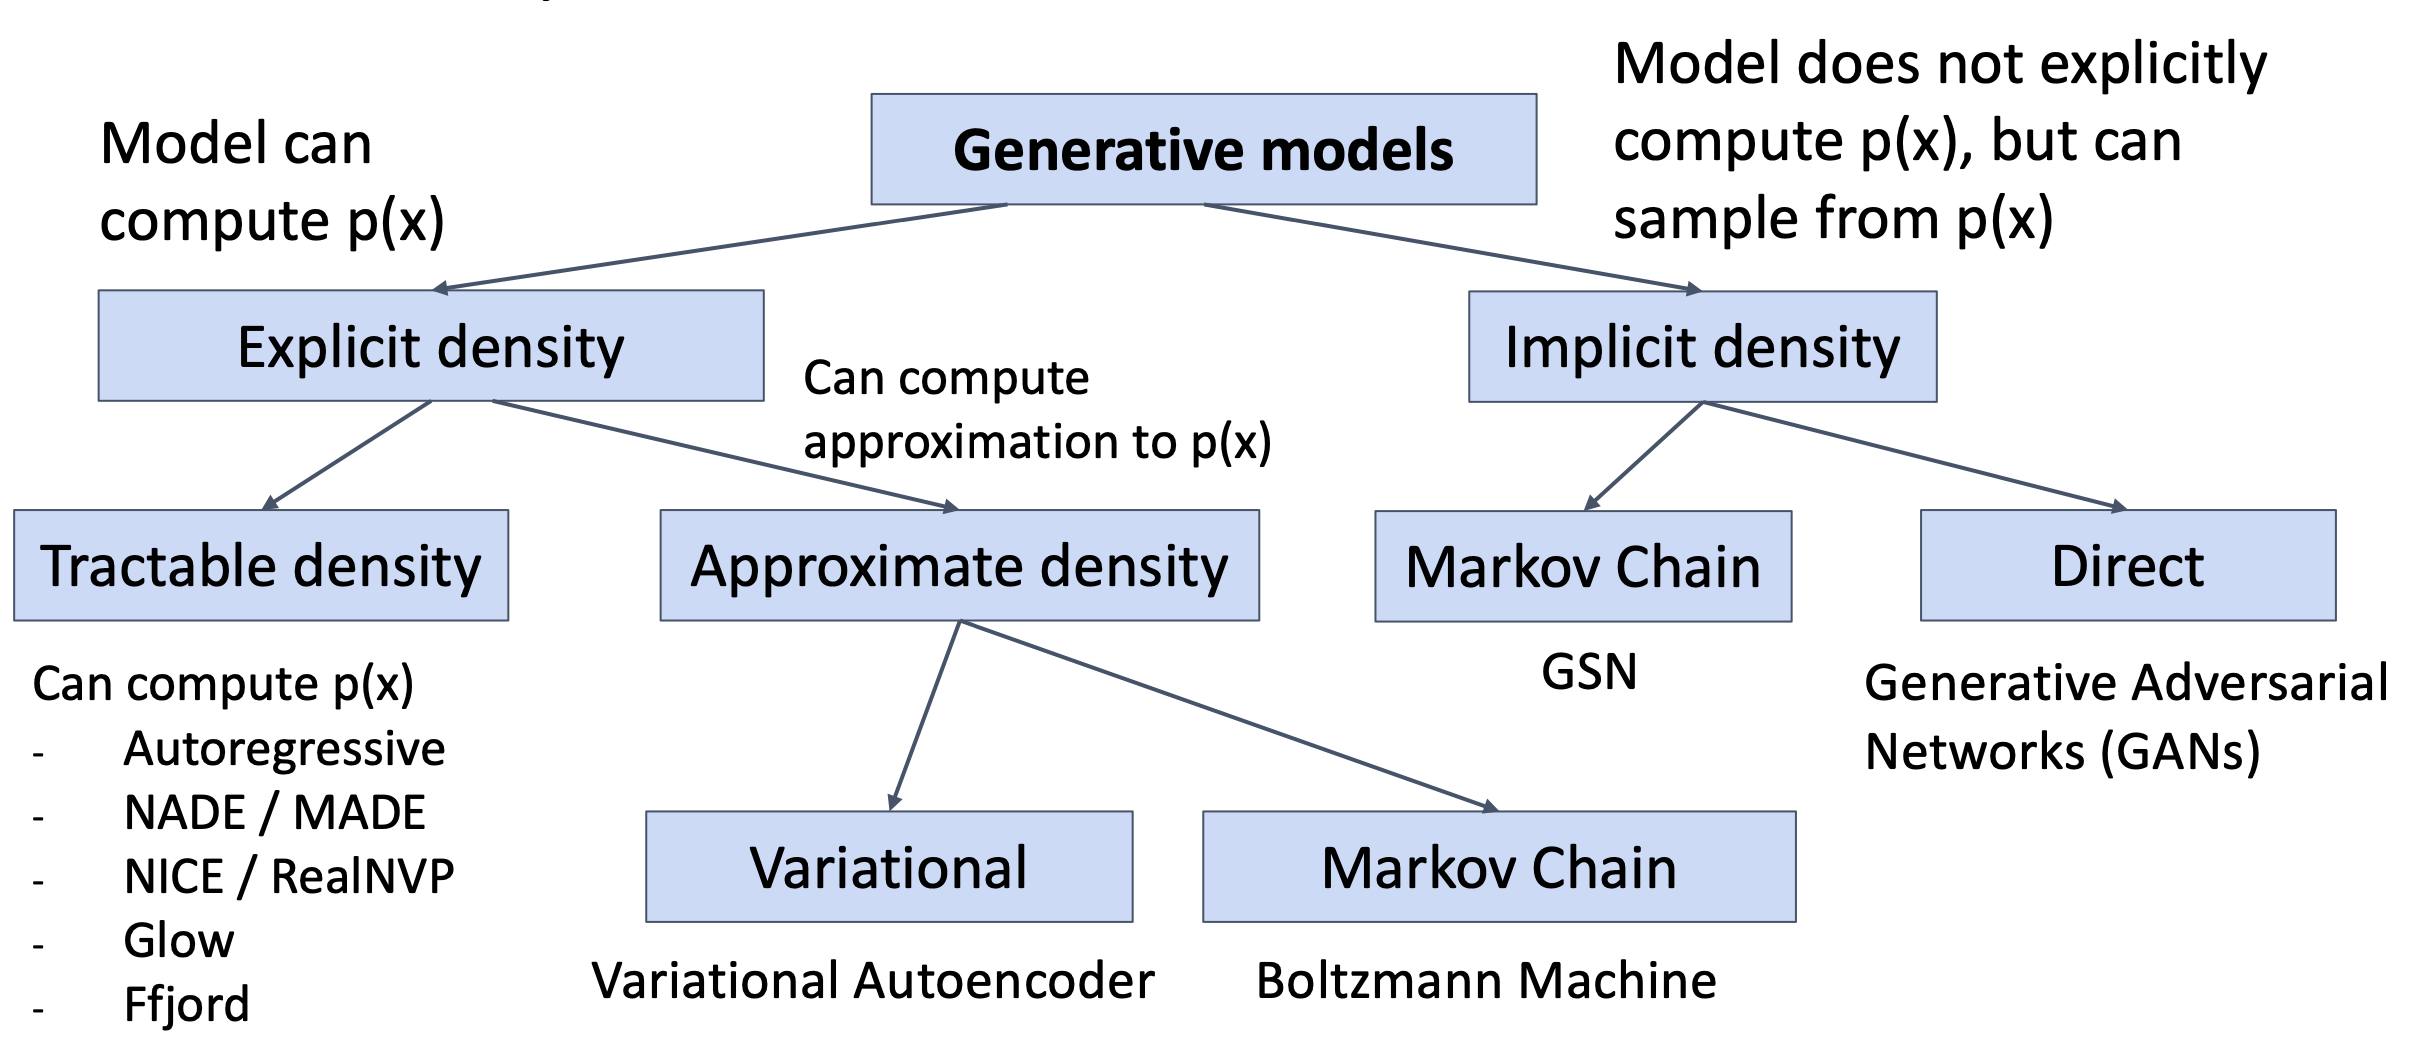
\includegraphics[width=.75\textwidth]{autoencoders/taxonomy-generative.png}
    \caption{Taxonomy of generative models}
\end{figure}
In this chapter, we will study an explicit and tractable density model family, the autoregressive models. In the next chapters, we will introduce Variational Autoencoders and Generative Adversarial Networks.

\subsection{Autoregressive Models}
\subsubsection{Explicit density estimation}
Our goal is to write an explicit function for the likelihood $\P(x)$, that is to find a parametric function $f_\theta$ such that for a certain learned value of $\theta^*$,
\begin{equation*}
    \forall x,\quad \P(x) = f_{\theta^*}(x)
\end{equation*}
Given a label-less dataset $(x^{(1)}, \dots, x^{(N)})$, we can train the model by solving the equation:
\begin{equation*}
    \begin{aligned}
        \theta^* &:= \argmax_\theta \prod_{i=1}^N \P(x^{(i)})\\
        &= \argmax_\theta \sum_{i=1}^N \log\P(x^{(i)})\\
        &= \argmax_\theta \sum_{i=1}^N \log f_\theta(x^{(i)})
    \end{aligned}
\end{equation*}
corresponding to maximum likelihood estimation. Therefore, we can simply take:
\begin{equation*}
    \L : \theta \longmapsto \sum_{i=1}^N \log f_\theta(x^{(i)})
\end{equation*}
as a loss function, and minimize it using gradient descent. In most practical applications, $\left(f_\theta\right)_\theta$ is a family of neural networks.

\subsubsection{Explicit density estimation using a regressive model}
The specificity of autoregressive models is to assume that each training sample $x^{(i)}$ consists of multiple subparts $(x_1^{(i)}, x_2^{(i)}, \dots, x_T^{(i)})$. For instance, in the case of images, each subpart can be a specific pixel.

We can break down the probability of observing a specific input by using the probability chain rule:
\begin{equation*}
    \begin{aligned}
        \P(x) &= \P(x_1, x_2, \dots, x_T)\\
        &= \P(x_1) \cdot \P(x_2|x_1) \cdot \P(x_3|x_1, x_2)\cdot \dots\\
        &= \prod_{t=1}^T \P(x_t|x_1, \dots, x_{t-1})
    \end{aligned}
\end{equation*}
This type of dependency is extremely similar to the problem solved by recurrent neural network: we want each prediction $\P(x_t|x_1, \dots, x_{t-1})$ to be conditioned on the previous time steps $x_1, \dots, x_{t-1}$. Therefore, we can train a recurrent neural network to output the successive probabilities $\P(x_t|x_1, \dots, x_{t-1})$ in a meaningful order, which can then be multiplied to obtain $\P(x)$.

\subsubsection{PixelRNN}
This is the idea of a PixelRNN: a generative model with an explicit and tractable density function, that predicts pixel values one at a time.

For each pixel, we compute a hidden state of the RNN, that depends on the hidden states and RGB values of pixels left and above:
\begin{equation*}
    h_{x,y} = f_\theta(h_{x-1,y}, h_{x, y-1})
\end{equation*}
That way, each pixel depends implicitly on all pixels left and above.
At each pixel, we can then predict the red, green, and blue values, by computing a probability distribution over $\iset{0}{255}$.
\begin{figure}[H]
    \centering
    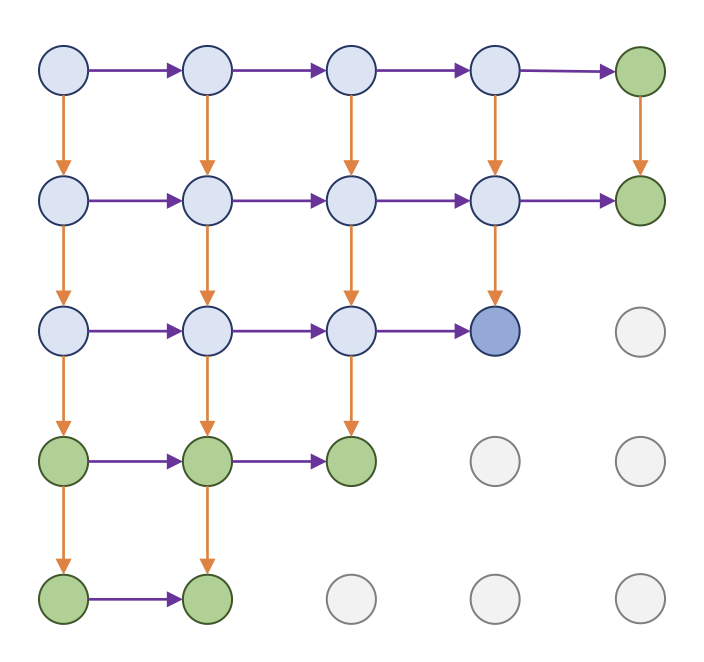
\includegraphics[width=.4\textwidth]{autoencoders/pixelrnn.png}
    \caption{Dependency of pixels in PixelRNN.}
\end{figure}

The major issue of this generative approach is that is it very slow both during training and testing.

\subsubsection{PixelCNN}
To overcome the performance issues of PixelRNN, another architecture called PixelCNN has been introduced: it still generates pixels from the top-left corner, but the dependency on each pixel is now modeled using a masked convolution over previously computed regions.
\begin{figure}[H]
    \centering
    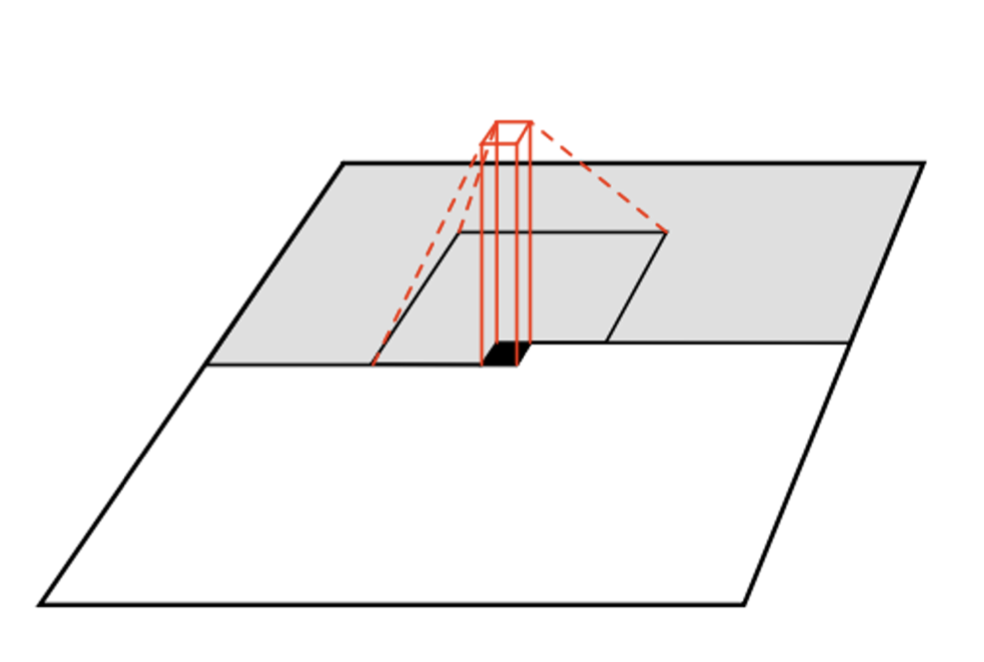
\includegraphics[width=.5\textwidth]{autoencoders/pixelcnn.png}
    \caption{Dependency of pixels in PixelCNN.}
\end{figure}
This approach allows for parallel computations of dependencies over previous pixels, making it much faster to train. It remains quite slow, because the generation must still proceed sequentially.

Generated result show that the model learned the high-level structure of the input images, by providing features such as edges and flat color shapes, but the images do not represent anything real when looked closely.\begin{figure}[H]
    \centering
    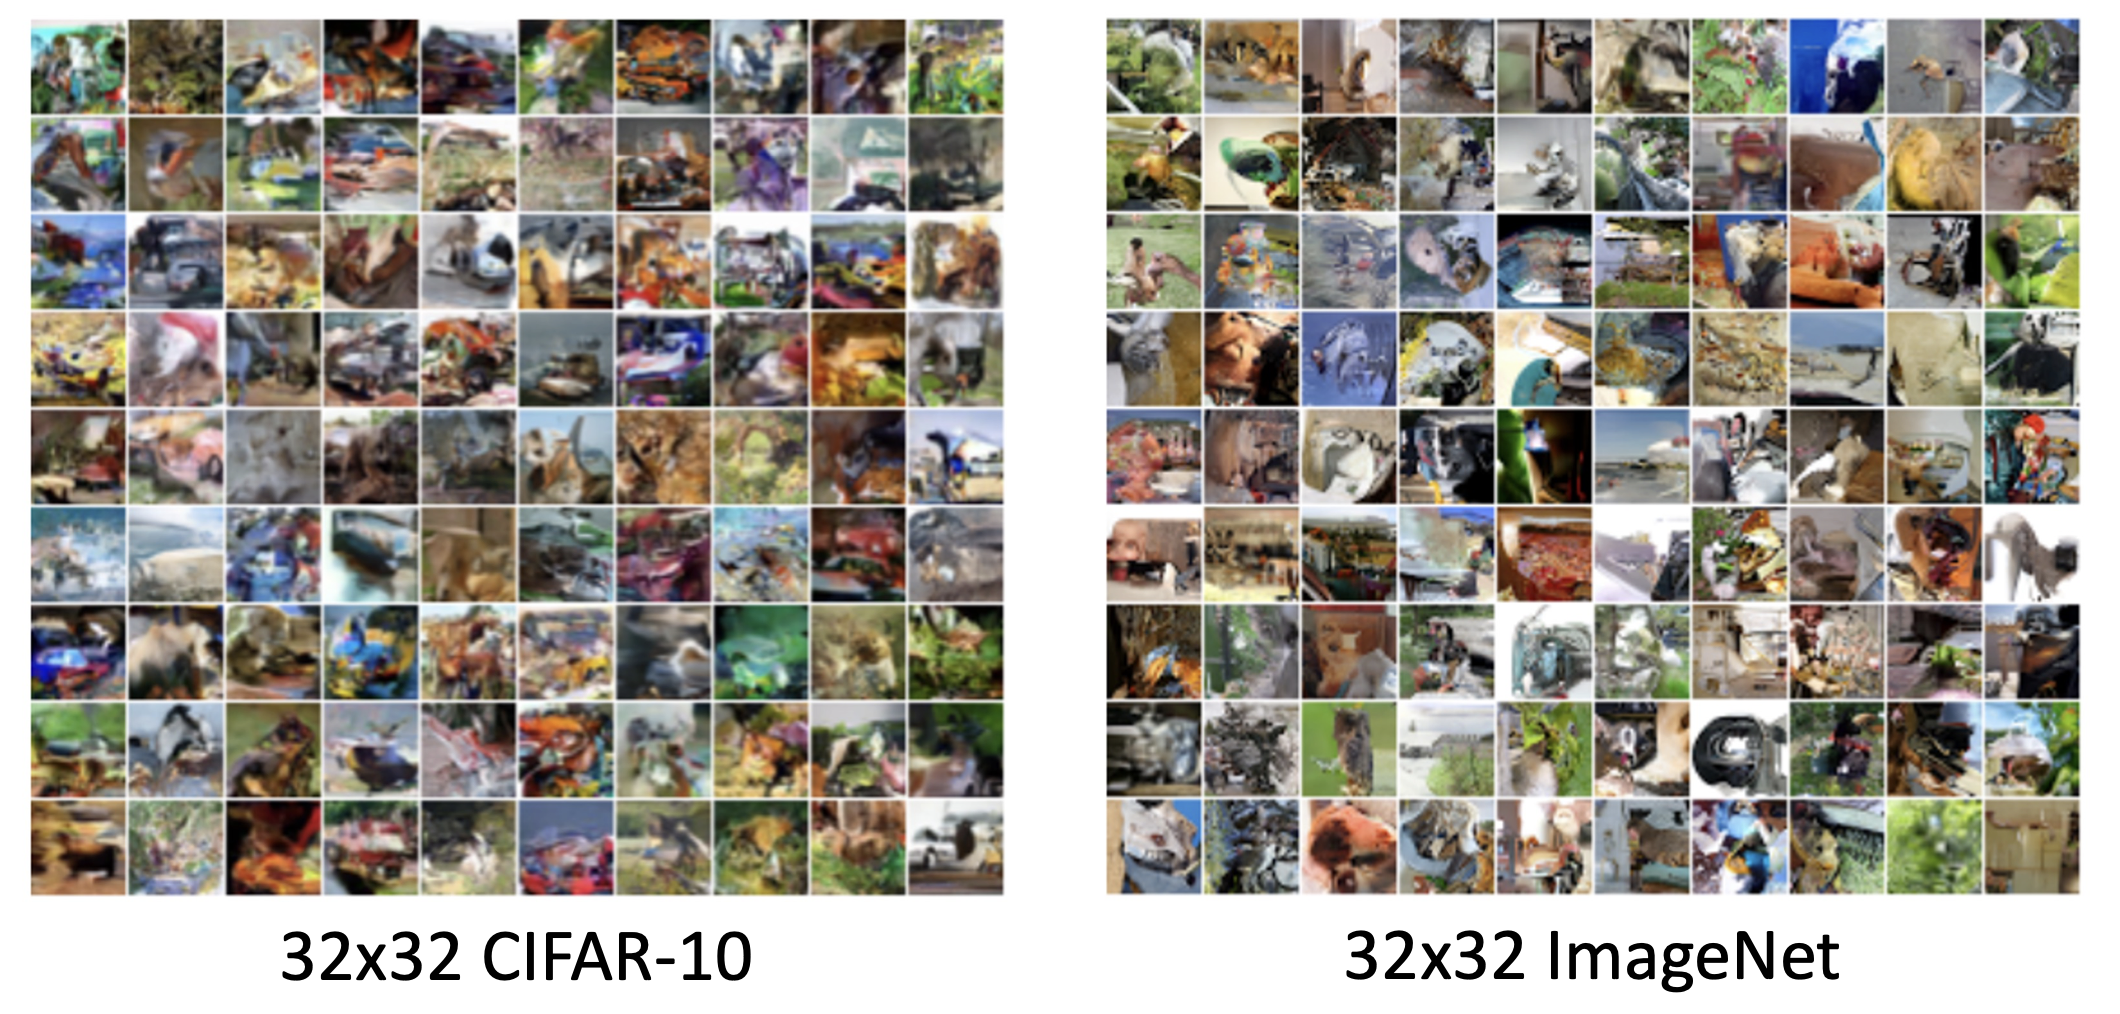
\includegraphics[width=.8\textwidth]{autoencoders/pixelcnn-results.png}
    \caption{Results of PixelCNN.}
\end{figure}

\subsubsection{Beyond autoregressive models}
Autoregressive models have the benefit of explicitly computing the likelihood $\P(x)$, making them very easy to evaluate. Nevertheless, they require a sequential generation, making the sampling process slow.

The performance of PixelCNN can be improved with tricks in practice, such as the use of multiscale generation, gated convolutional layers or shortcut connections.

\newpage
\section{Autoencoders}
An \emph{autoencoder} is a type of neural network used to solve unsupervised learning problems. The main idea of an autoencoder is to learn an efficient representation of the input data, usually of the form of a hidden layer of size smaller than the input size. It can be useful in dimensionality reduction, but the mostly used variant is the \emph{variational autoencoder}, a certain type of generative model.

\subsection{Regular Autoencoders}
\subsubsection{Principle}
Autoencoders are designed to learn feature vectors from raw data, without any labels. Features should extract useful information, that we can use for other tasks. The main challenge is to learn this feature transform from raw data, without any idea of the form that this feature vector should take. Therefore, the idea of autoencoders is to ask the model to use these features to estimate the raw data; this way, the model will keep the features that will help it reconstruct the data, which can be intuitively considered as the \say{best} features.

An autoencoder consists of two parts: an encoder, taking into input the raw data $x$ and outputing the feature vector $z$; and a decoder, taking the feature vector $z$ as input and outputing the reconstructing input data $\hat{x}$. Both the encoder and the decoder are updated during training; the name \emph{autoencoder} shows that the model chooses its own code.
\begin{figure}[H]
    \centering
    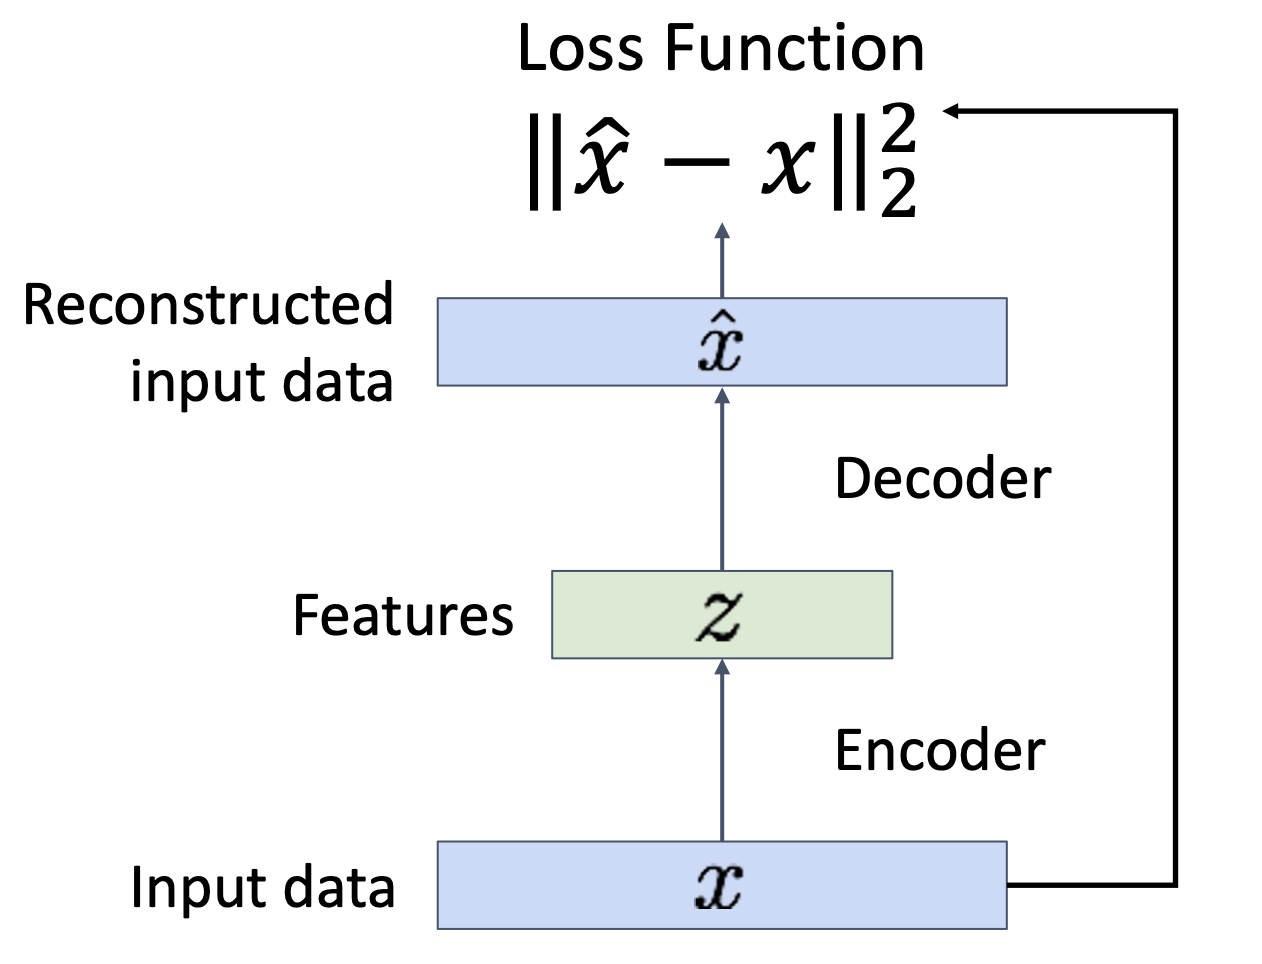
\includegraphics[width=.6\textwidth]{autoencoders/encoder-decoder.png}
    \caption{The encoder-decoder architecture of an autoencoder.}
\end{figure}
Since the goal of the decoder is to reconstruct the input data as well as possible, our loss function will be the difference between the input and the output data:
\begin{equation*}
    \L(x) = \norm{\hat{x}-x}_2^2 = \norm{f_\theta(x)-x}_2^2
\end{equation*}

In general, learning the identity function is not especially usefull and can be easily learned by a simple neural network. Therefore, features need to have a low dimension compared to the data, and act as a bottleneck. If the model approximates the identity function well, it means that the latent code (the feature vector) is an efficient way to represent the input data.

\subsubsection{Applications}
Once trained, the encoder part can be extracted and added upstream of another supervised model to solve other problems: for instance, we might add a classifier downstream and fine-tune the encoder and the classifier together.
\begin{figure}[H]
    \centering
    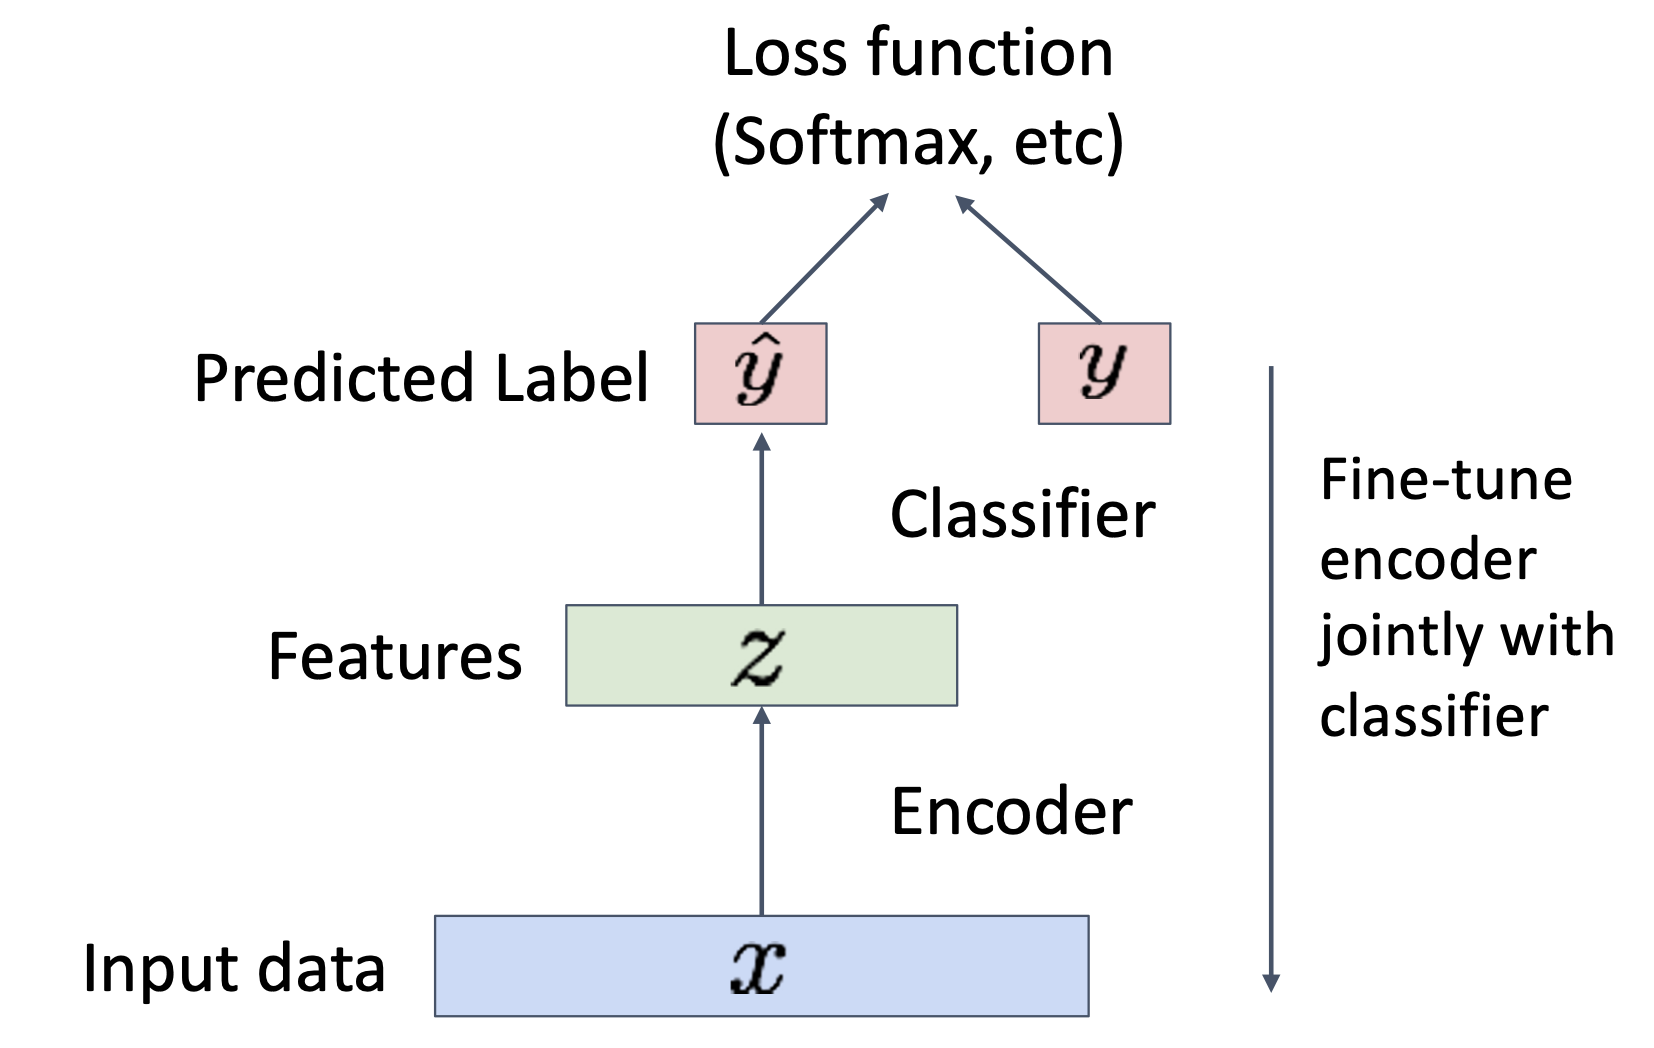
\includegraphics[width=.6\textwidth]{autoencoders/encoder-classifier.png}
    \caption{Use of the trained encoder for a downstream classification task.}
\end{figure}
One could think that we could directly train the encoder from scratch along with the classifier. In practice, training an encoder inside an autoencoder produces better results: since the autoencoder does not need labeled data, it is very simple to train on a huge amount of unlabeled inputs, producing a more robust and performant encoder.

\subsection{Variational Autoencoders}
\subsubsection{Probabilistic modelling}
We would like to adapt the autoencoder formalism to generate new inputs. Regular autoencoders are not probabilistic, and can only be used to generate the latent features $z$ of an input $x$. Instead, \emph{Variational Autoencoders} (VAEs) will be used to learn a probability distribution, from which we can sample new data.

Formally, we assume that our training data $(x^{(i)})_{i\in\iset{1}{N}}$ is generated from a latent representation $z$, to which we do not have access to. After training, the variational autoencoder will proceed in two steps to output a probability distribution over new inputs. First, it will sample a certain feature vector $z$ from some learned prior distribution $\P_{\theta^*}(z)$. Then, it will use this generated latent representation to output the conditional probability distribution $\P_{\theta^*}(x|z)$.
\begin{figure}[H]
    \centering
    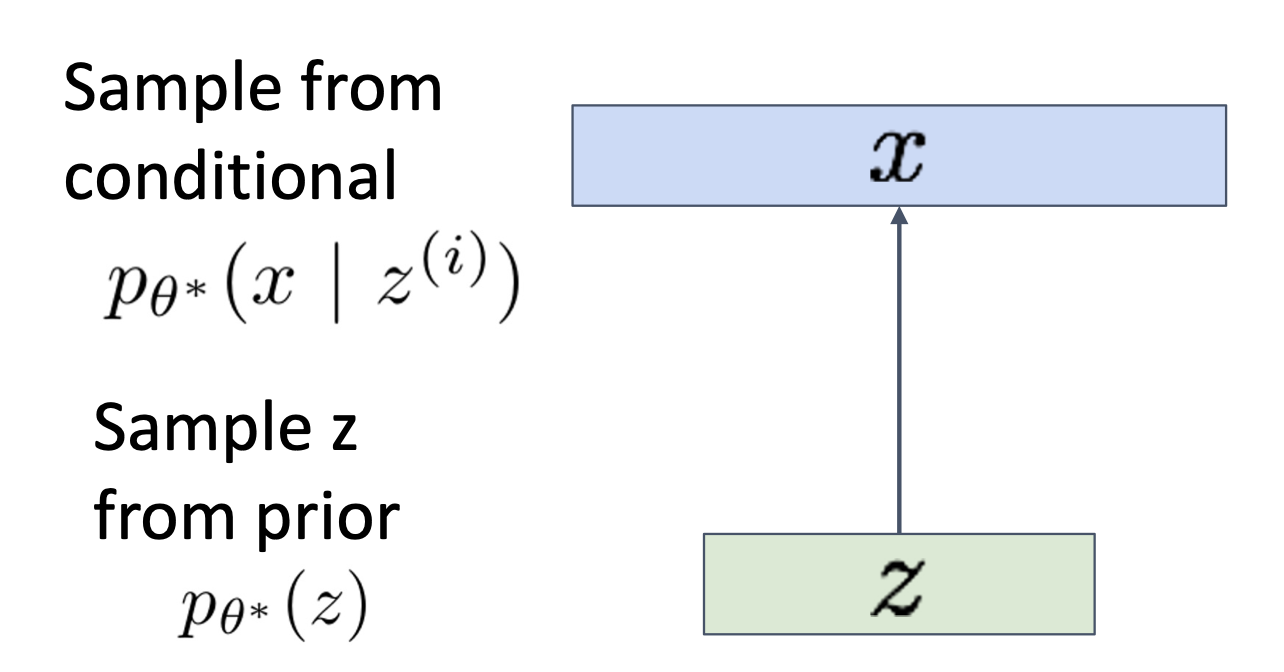
\includegraphics[width=.5\textwidth]{autoencoders/variational-principle.png}
\end{figure}

The prior distribution $\P_{\theta^*}(z)$ can be assumed to be very simple, such as a Gaussian distribution over $\R^d$. The conditional distribution $\P_{\theta^*}(x|z)$ will be represented with a neural network, similar to the decoder of an autoencoder. To do so, we will output the parameters of a parametrized output distribution. For instance, we can output a vector $\mu_{x|z}$ and a diagonal matrix $\Sigma_{x|z}$, and say that the associated distribution is the Gaussian distribution over $\R^d$ of mean $\mu_{x|z}$ and covariance matrix $\Sigma_{x|z}$.
\begin{figure}[H]
    \centering
    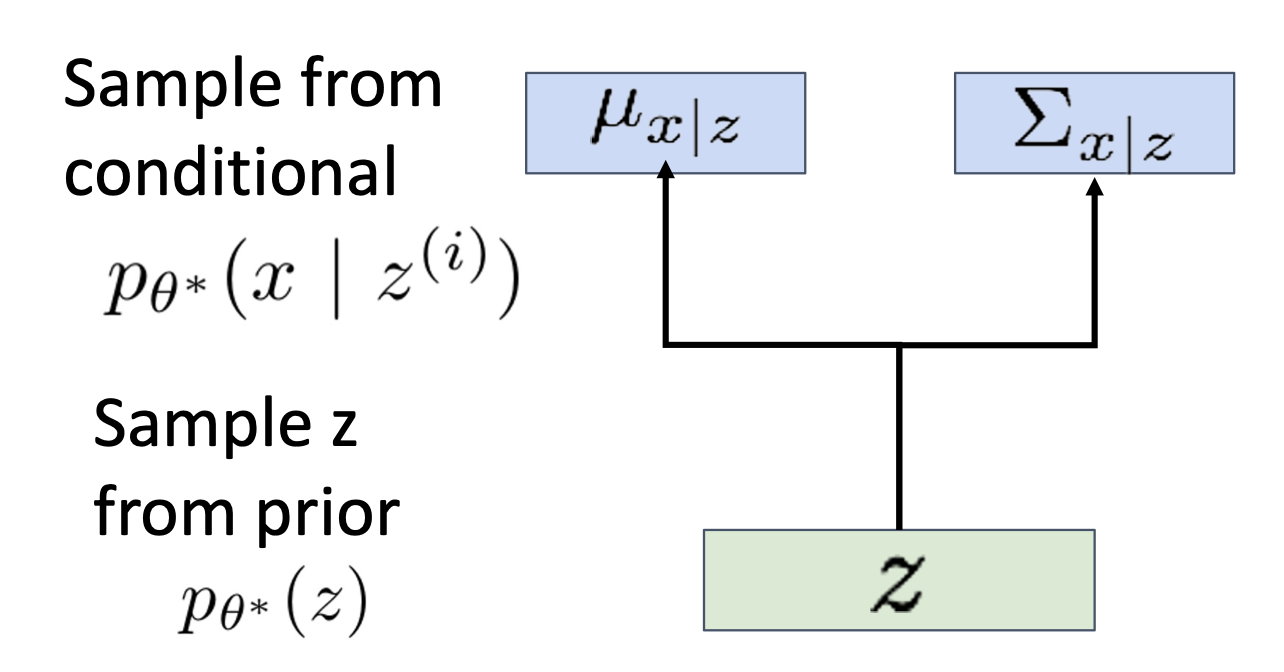
\includegraphics[width=.5\textwidth]{autoencoders/gaussian-parameters.png}
\end{figure}

\subsubsection{Variational lower bound}
To train the variational autoencoder, we maximize the likelihood of the data. Given the latent vectors $(z^{(i)})_{i\in\iset{1}{N}}$, we could train the conditional generative model part directly, but we do not have access to $z$. Therefore, we will jointly train two parts, just like for regular autoencoders: an encoder that inputs data $x$, and outputs a distribution over the latent codes $z$, and a decoder that inputs a latent code $z$ and outputs a distribution over the data $x$.

\begin{figure}[H]
    \centering
    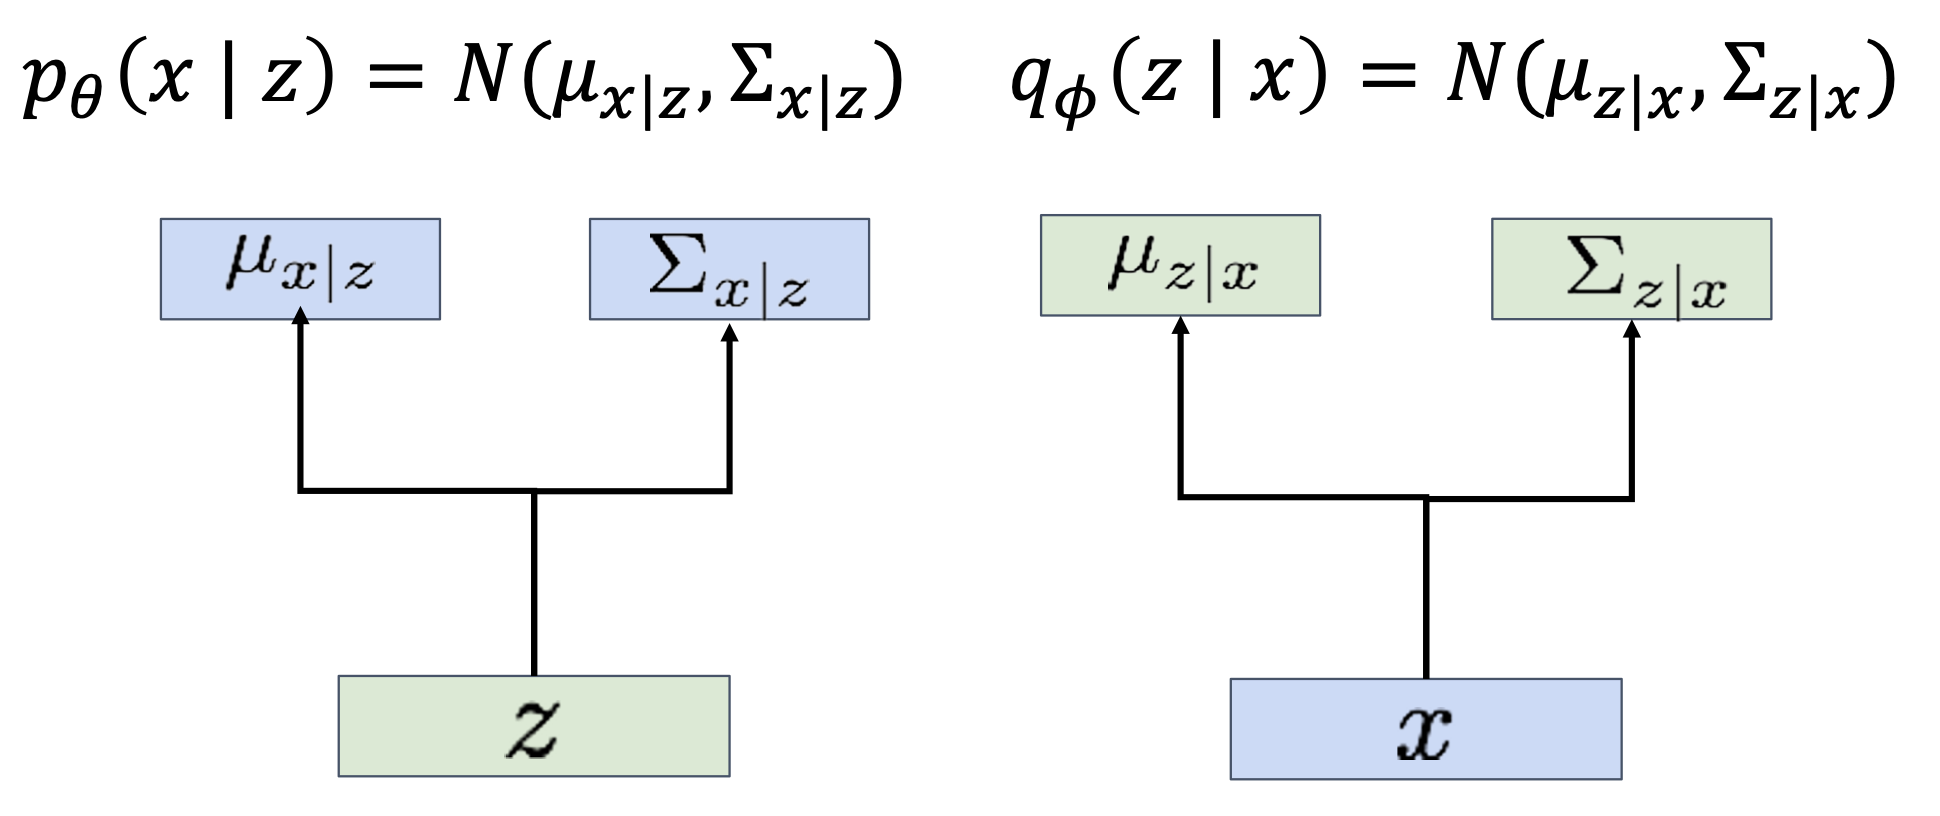
\includegraphics[width=.6\textwidth]{autoencoders/variational-encoder-decoder.png}
\end{figure}

Note that according to Bayes' rule:
\begin{equation*}
    \P_\theta(x) = \frac{\P_\theta(x|z)\cdot \P_\theta(z)}{\P_\theta(z|x)}
\end{equation*}
The probability $p_\theta(x|z)$ is computed by the network taking into input $z$ and outputing the Gaussian parameters. We assumed $z$ to be sampled from a Gaussian distribution, we therefore know $\P_\theta(z)$. Finally, $\P_\theta(z|x)$ is estimated by the encoder.

\begin{property}[Variational lower bound]
    The following inequality holds for any distributions $p_\theta$ and $q_\varphi$:
    \begin{equation}
        \label{eq:variational-lower-bound}
        \log p_\theta(x) \geq \E_{z\sim q_\varphi(z|x)}\left[\log p_\theta(x|z)\right] - \KL\left(q_\varphi(z|x)\parallel p_\theta(x)\right)
    \end{equation}
    where $\KL$ denotes the Kullback-Leibler divergence.
\end{property}
\begin{proof}
    We decompose $p_\theta(x)$:
    \begin{align*}
        \log p_\theta(x) &= \log\frac{p_\theta(x|z)\cdot p(z)}{p_\theta(z|x)} && \text{(Bayes' rule)} \\
        &= \log\frac{p_\theta(x|z)\cdot p(z)\cdot q_\varphi(z|x)}{p_\theta(z|x)\cdot q_\varphi(z|x)} \\
        &= \log p_\theta(x|z) - \log\frac{q_\varphi(z|x)}{p(z)} + \log\frac{q_\varphi(z|x)}{p_\theta(z|x)} \\
        &= \E_{z\sim q_\varphi(z|x)}\left[\log p_\theta(x|z)\right] - \E_{z\sim q_\varphi(z|x)}\left[\log\frac{q_\varphi(z|x)}{p(z)}\right] + \E_{z\sim q_\varphi(z|x)}\left[\log\frac{q_\varphi(z|x)}{p_\theta(z|x)}\right] \\
        &= \E_{z\sim q_\varphi(z|x)}\left[\log p_\theta(x|z)\right] - \KL\left(q_\varphi(z|x)\parallel p(z)\right) + \KL\left(q_\varphi(z|x)\parallel p_\theta(z|x)\right)
    \end{align*}
    Since the Kullback-Leibler divergence is always positive, we can ommit the rightmost term and obtain:
    \begin{equation*}
        \log p_\theta(x) \geq \E_{z\sim q_\varphi(z|x)}\left[\log p_\theta(x|z)\right] - \KL\left(q_\varphi(z|x)\parallel p_\theta(x)\right)
    \end{equation*}
\end{proof}

We will train the encoder and decoder of the variational autoencoder by maximizing the \emph{Evidence Lower Bound} \autoref{eq:variational-lower-bound}.

% TODO: move this subsubsection and the next one before variational lower bound?
\subsubsection{Example: Fully-connected Variational Autoencoder}
To give a concrete example, let's imagine that we want to train a variational autoencoder on the MNIST dataset to generate new images. The input data $x$ is a flatted $28\times28$ image, therefore $x\in\R^{784}$; we choose the latent space to be $z\in\R^{20}$. We choose both the encoder and the decoder network to be fully-connected networks as described in \autoref{fig:fully-connected-vae}.
\begin{figure}[H]
    \centering
    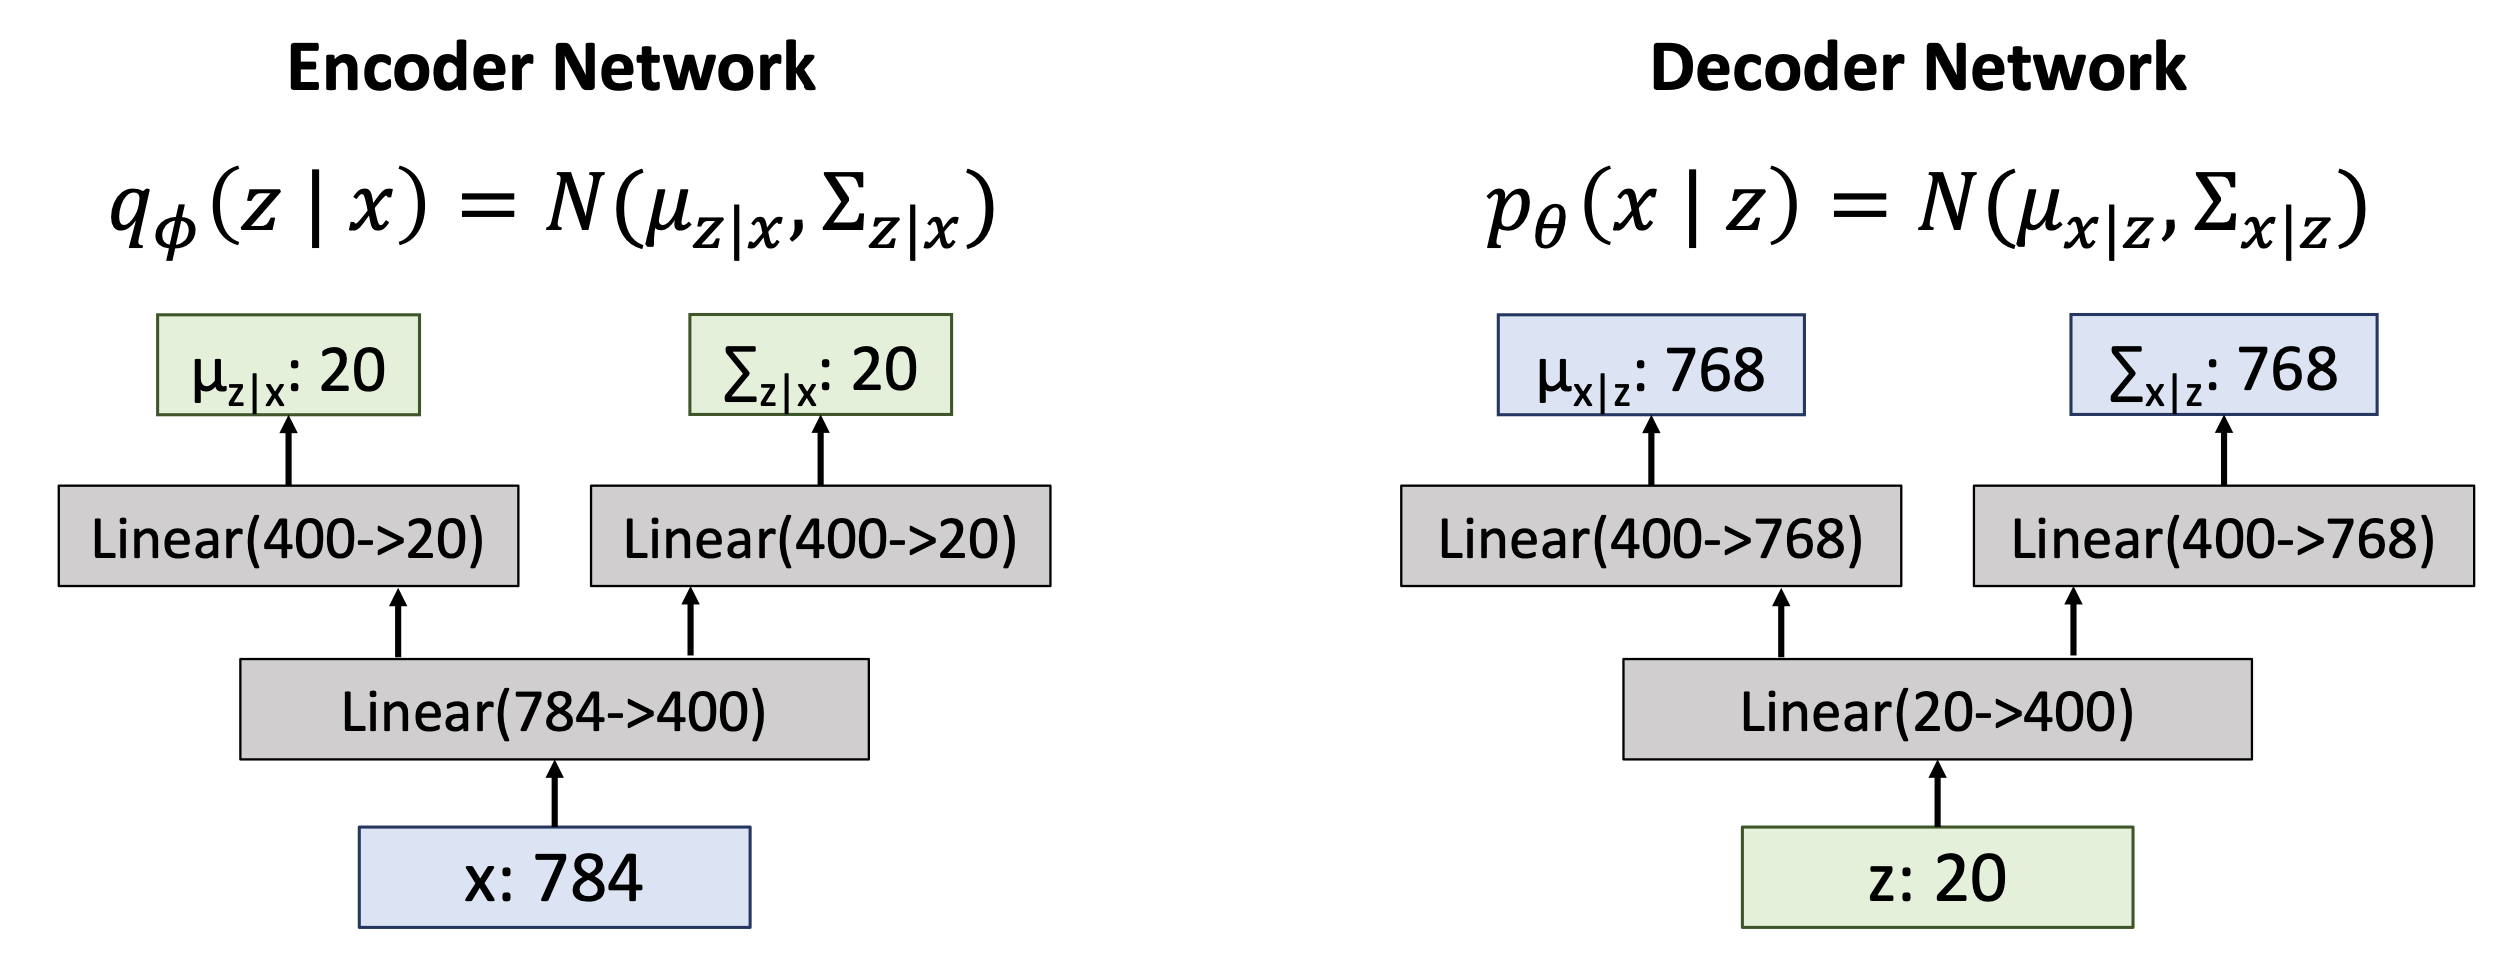
\includegraphics[width=.8\textwidth]{autoencoders/fully-connected-vae.png}
    \caption{A fully-connected variational autoencoder.}
    \label{fig:fully-connected-vae}
\end{figure}

\subsubsection{Forward pass during training}
The forward pass of a variational autoencoder is very similar to the one of a regular autoencoder, except that both the encoder and the decoder output Gaussian parameters. Therefore, we can compute the output data distribution in three simple steps:
\begin{itemize}
    \item First, we feed the input data $x$ to the encoder, which outputs the mean $\mu_{z|x}$ and the diagonal covariance matrix $\Sigma_{z|x}$ of the latent distribution.
    \item Then, we sample a latent vector $z$ from this distribution $\Nc(\mu_{z|x}, \Sigma_{z|x})$.
    \item Finally, we feed this latent vector to the decoder, which outputs the mean $\mu_{x|z}$ and the diagonal covariance matrix $\Sigma_{x|z}$ of the output distribution.
\end{itemize}
We can then sample a new data point $\hat{x}$ from this distribution $\Nc(\mu_{x|z}, \Sigma_{x|z})$.
\begin{figure}[H]
    \centering
    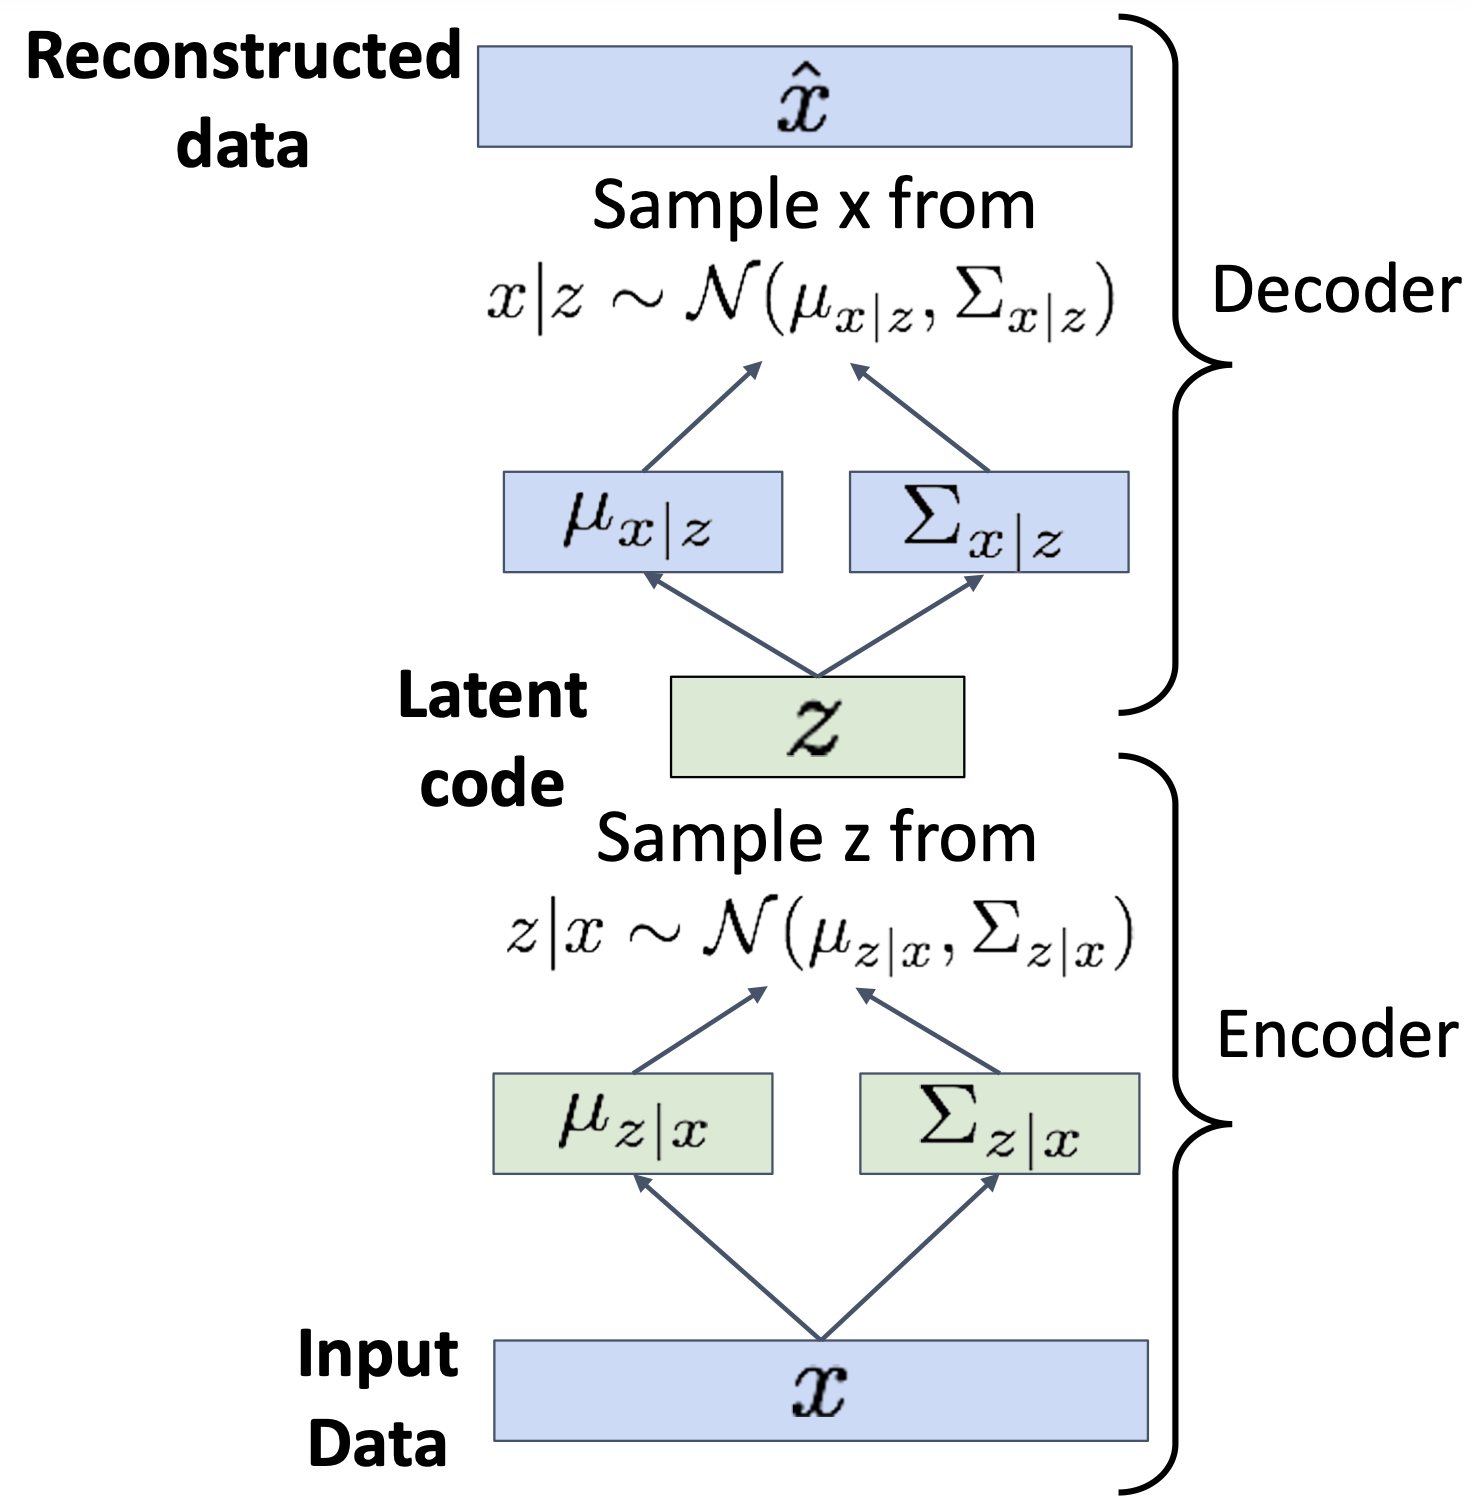
\includegraphics[width=.55\textwidth]{autoencoders/vae-training.png}
    \caption{The successive steps of a forward pass of a VAE during training.}
\end{figure}


\subsubsection{Loss computation during training}
Recall that to train the model, we will maximize the lower bound of the probability:
\begin{equation*}
    \L(x) = \E_{z\sim q_\varphi(z|x)}\left[\log p_\theta(x|z)\right] - \KL\left(q_\varphi(z|x)\parallel p_\theta(x)\right)
\end{equation*}
The two terms of this loss function can be computed during the forward pass of the model. Given the distribution over $z$, the Kullback-Leibler divergence term can be computed analytically, since we assumed a simple form for the prior distribution -- a unit Gaussian. The first term -- the expectation -- can be computed by sampling $z$ and computing the $\log$-likelihood of the output data given this latent vector.

More specifically, the KL term can be computed as:
\begin{equation*}
    \begin{aligned}
        -\KL\left(q_\varphi(z|x)\parallel p(z)\right) &= \int_z q_\varphi(z|x)\cdot\log\frac{p(z)}{q_\varphi(z|x)}\dd z\\
        &= \int_z N(z; \mu_{z|x}, \Sigma_{z|x})\cdot\log\frac{N(z; 0, I_d)}{N(z; \mu_{z|x}, \Sigma_{z|x})}\dd z\\
        &= \frac{1}{2}\sum_{k=1}^d \left(1 + \log\left(\Sigma_{z|x}\right)^2_j - \left(\mu_{z|x}\right)^2_j - \left(\Sigma_{z|x}\right)^2_j\right)
    \end{aligned}
\end{equation*}
where $N$ is the probability density of the Gaussian distribution\footnote{That is $N(z; \mu, \Sigma) = \frac{1}{(2\pi)^{d/2}|\Sigma|^{1/2}}\cdot\exp\left[-\frac{1}{2}(x-\mu)^\tp\Sigma^{-1}(x-\mu)\right]$}.

Note that the two terms of the loss function are competing against each other: the $\KL$ term encourages the latent distribution to be close to the prior distribution, while the $\E$ term encourages the model to generate data close to the input data.

\subsubsection{Generating new data}
After training, we can extract the decoder part of the model and use it to generate new data. To do so, we sample a latent vector $z$ from the prior distribution $p(z)$, and feed it to the decoder. The output of the decoder will be a distribution over the data, from which we can sample a new data point.
\begin{figure}[H]
    \centering
    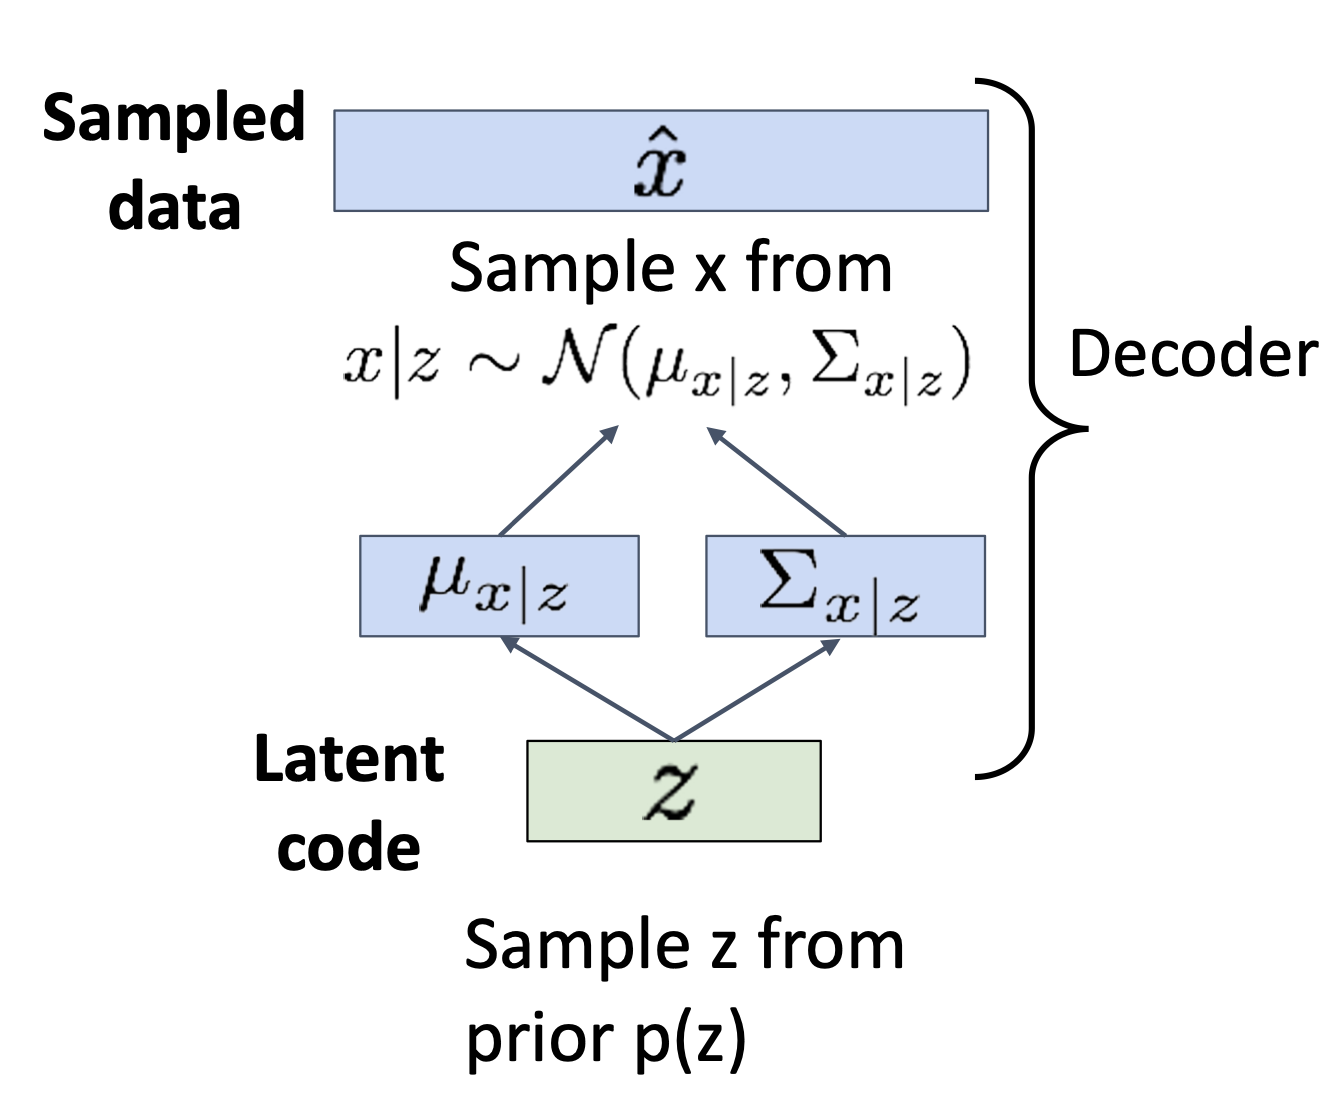
\includegraphics[width=.55\textwidth]{autoencoders/vae-generation.png}
    \caption{Steps to generate new data using a trained VAE.}
\end{figure}

Such models have been trained on different datasets, giving improved results compared to autoregressive models. The generated images are more realistic and have a better structure, as shown in the following figure.
\begin{figure}[H]
    \centering
    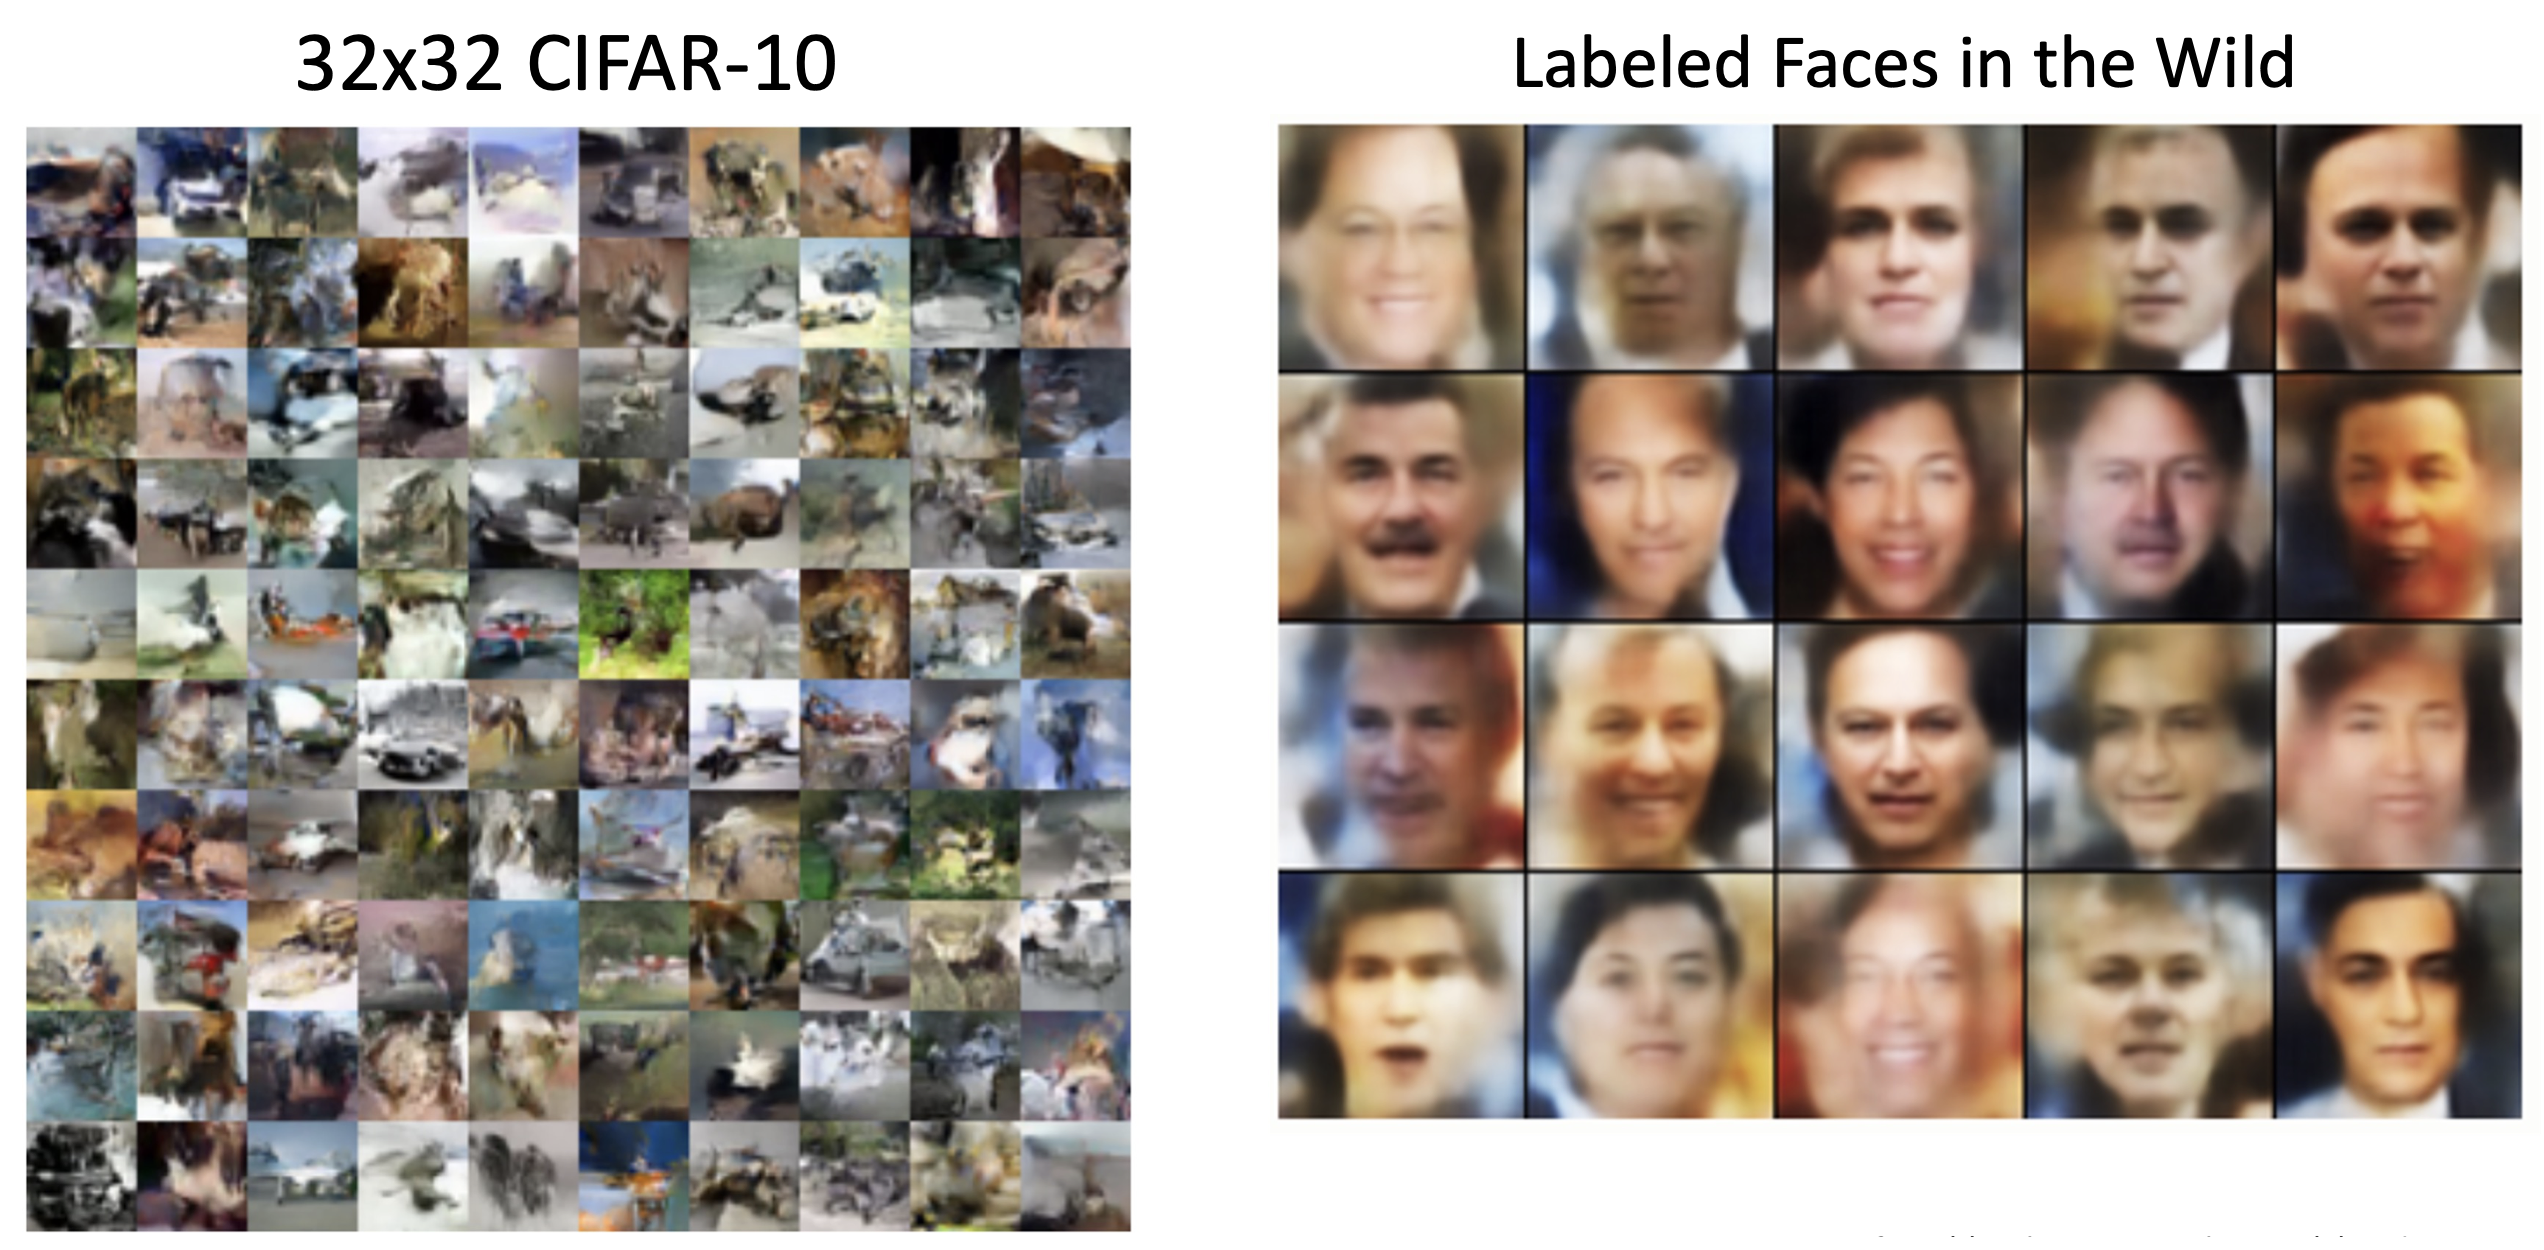
\includegraphics[width=.85\textwidth]{autoencoders/vae-images.png}
    \caption{Images generated by VAEs trained on different datasets.}
\end{figure}

Since we forced the latent space to be a diagonal Gaussian, the dimensions of $z$ are independent. Therefore, we can play around with the different coefficients of the latent feature vector to generate new data with specific features. This also shows that VAEs are not only learning to generate new data -- like autoregressive models -- but actually learn to generate data from a specific set of features, manifesting a deeper understanding of the data.

\subsubsection{Image editing using Variational Autoencoders}
The feature-level understanding of a trained VAE allows it to perform image editing tasks. The idea is to take an image, encode it to get the latent feature vector, modify this vector to change the features of the image, and then decode it to get the modified image. This can be used to perform tasks such as changing the color of an object, adding a smile to a face, or changing the orientation of an object.
\begin{figure}[H]
    \centering
    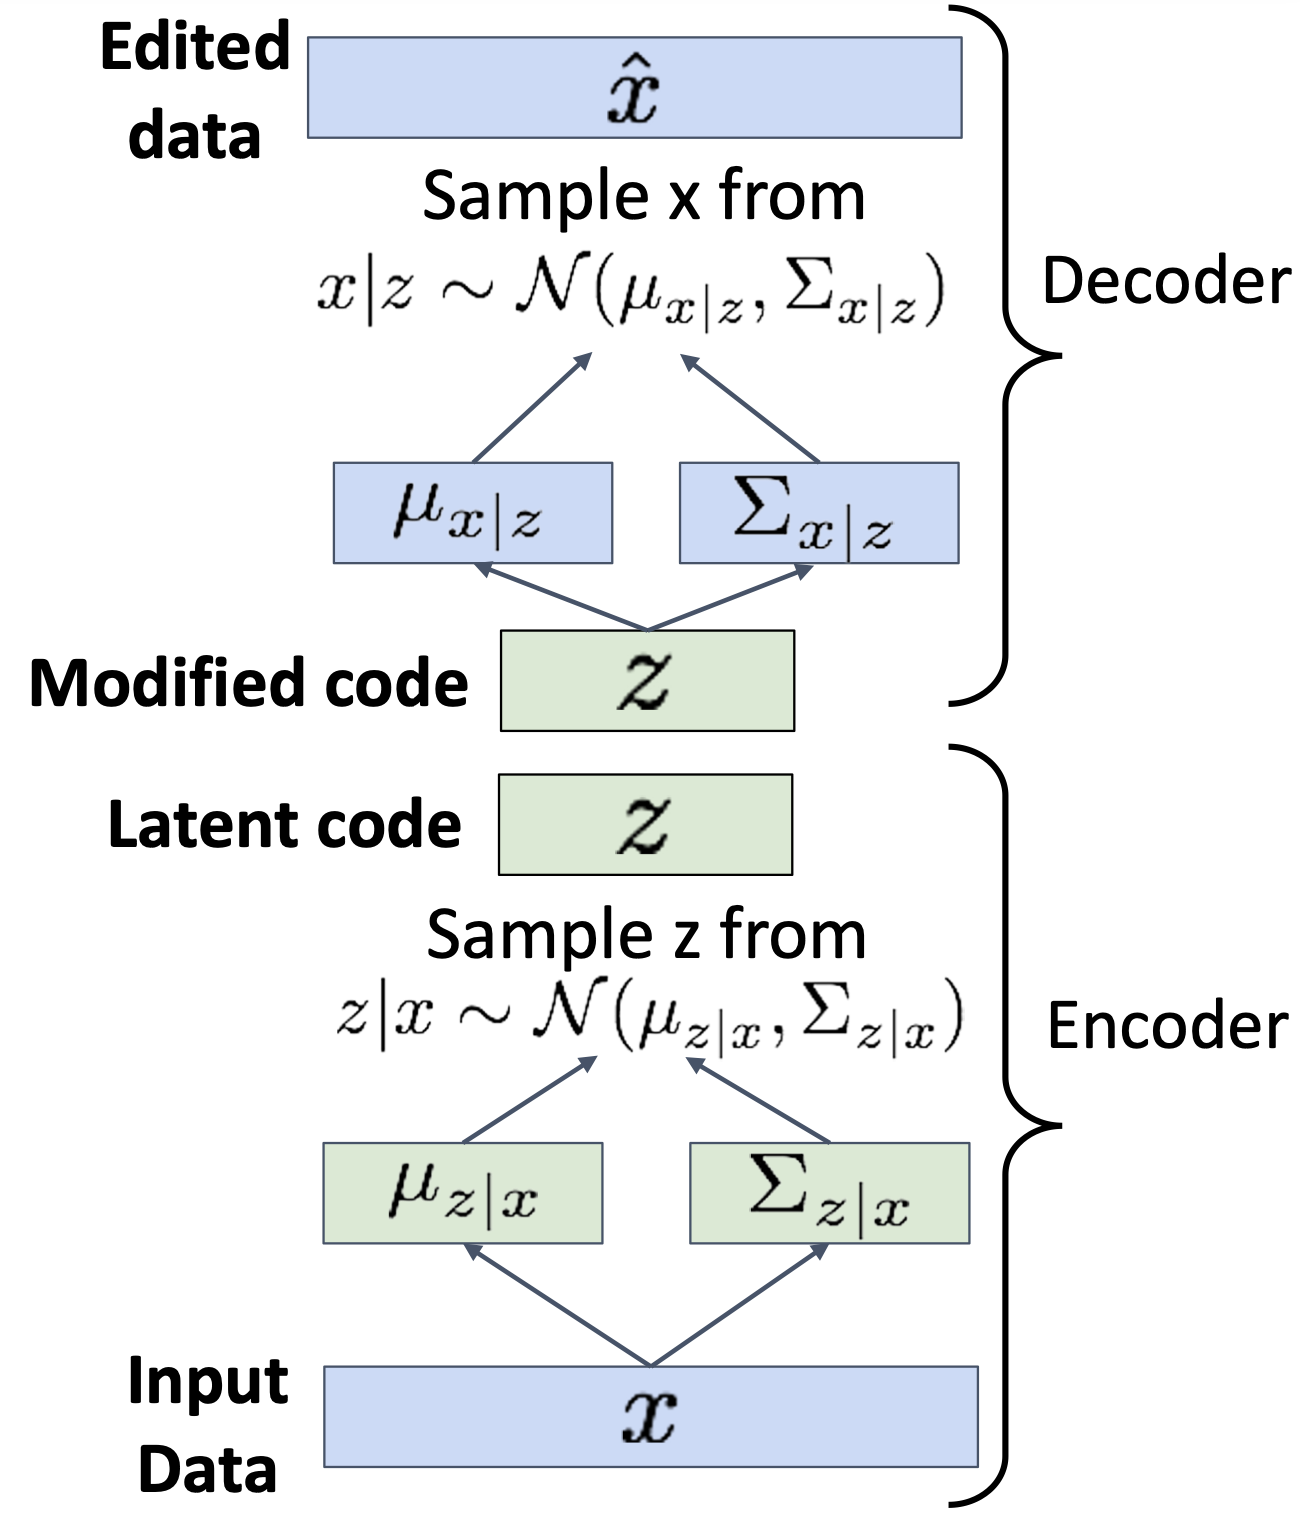
\includegraphics[width=.35\textwidth]{autoencoders/vae-image-editing.png}
\end{figure}

\begin{figure}[H]
    \centering
    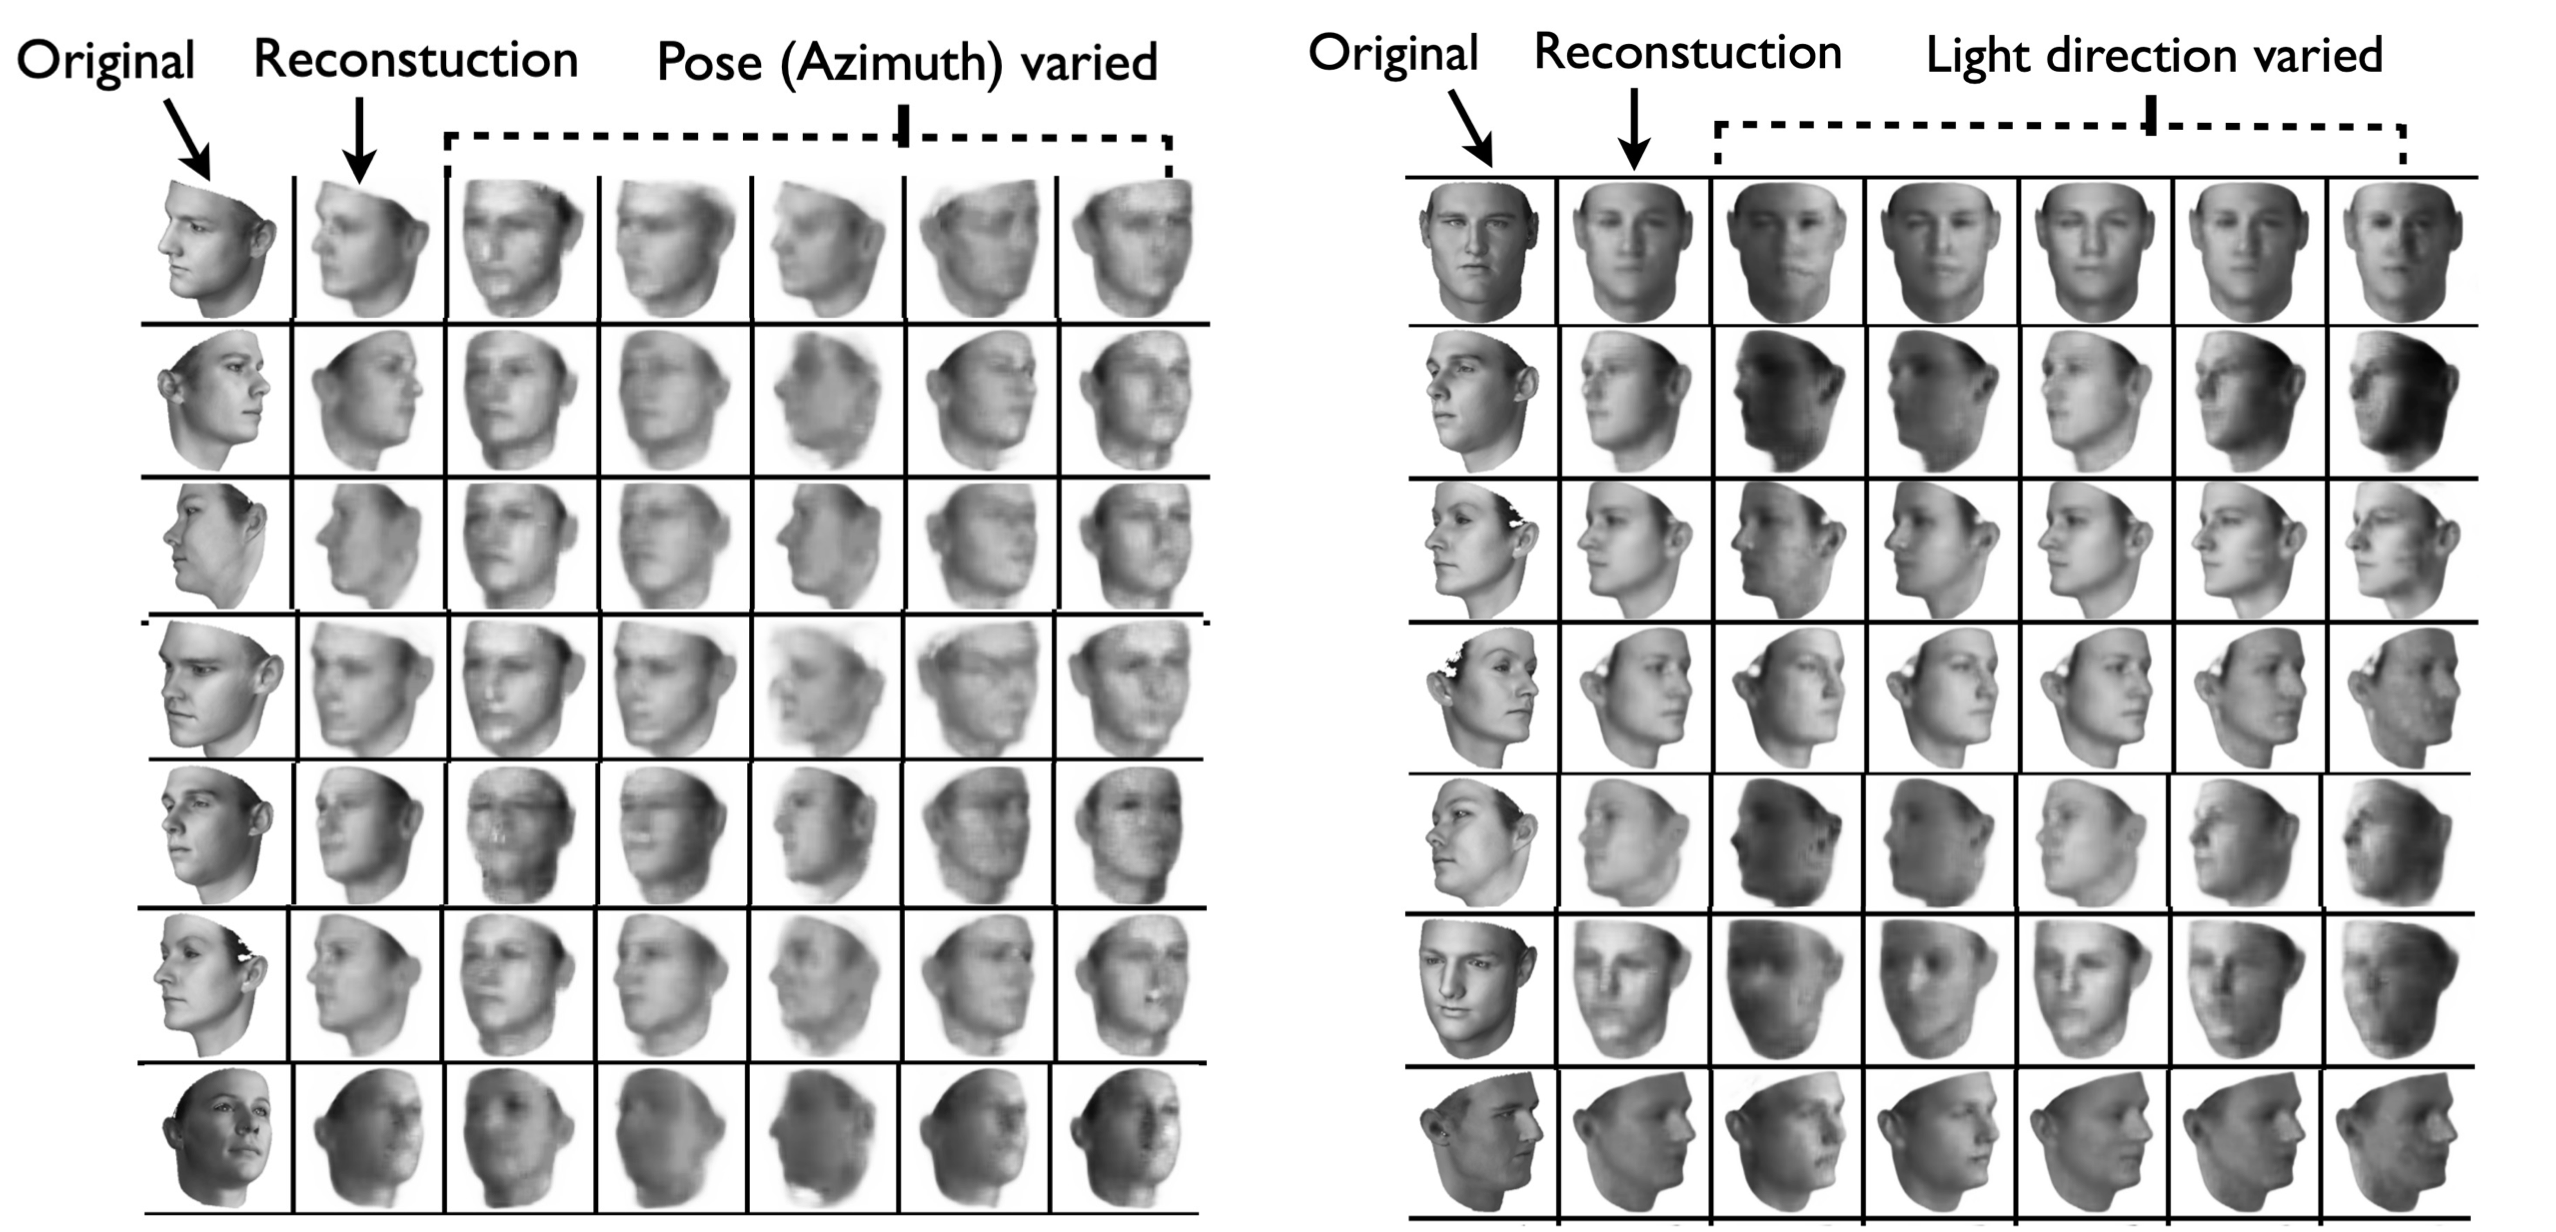
\includegraphics[width=.8\textwidth]{autoencoders/vae-sample-editing.png}
    \caption{Image editing using a trained VAE.}
\end{figure}

\subsection*{Autoencoders: Summary}
Regular autoencoders are networks composed of an encoder and a decoder, trained to learn the identity function despite a bottleneck between the encoder and the decoder.

Variational autoencoders is a generative variant of the regular autoencoders, that learns a probability distribution over the data. It is trained by maximizing a lower bound on the likelihood. It is a principled approach to generating new data, that learns a powerful feature-level representation of the data. Nevertheless, the fact that it maximizes a lower bound on the likelihood makes it less powerful than tractable generative models; it also produces samples that are blurrier and lower quality compared to the state-of-the-art, such as Generative Adversarial Networks.

\newpage